\documentclass[12pt,a4paper]{article}

% ─── Page Layout ───────────────────────────────────────────────────────────────
\usepackage[a4paper, margin=0.8in, headheight=14pt]{geometry}

% ─── Fonts (XeLaTeX) ───────────────────────────────────────────────────────────
\usepackage{fontspec}
\usepackage{unicode-math}
\setmainfont{TeX Gyre Pagella}
\setmonofont[Scale=0.88]{TeX Gyre Cursor}
\setmathfont{Latin Modern Math}

% ─── Packages ──────────────────────────────────────────────────────────────────
\usepackage{xcolor}
\usepackage{colortbl}
\usepackage{titlesec}
\usepackage{enumitem}
\usepackage{tabularx}
\usepackage{booktabs}
\usepackage{array}
\usepackage{amsmath}
\usepackage{tikz}
\usetikzlibrary{shapes.geometric, arrows.meta, positioning, calc, fit, decorations.pathreplacing}
\usepackage{tcolorbox}
\tcbuselibrary{skins, breakable}
\usepackage{hyperref}
\usepackage{fancyhdr}
\usepackage{graphicx}
\usepackage{microtype}
\hyphenpenalty=10000
\exhyphenpenalty=10000
\sloppy
\usepackage{caption}
\usepackage{setspace}
\usepackage{multirow}
\usepackage{tocloft}

% ─── Q&A helper ────────────────────────────────────────────────────────────────
\newcommand{\Q}[1]{\textbf{#1}\par\noindent\ignorespaces}

% ─── Colour Palette ────────────────────────────────────────────────────────────
\definecolor{myred}{RGB}{196,30,58}
\definecolor{mydark}{RGB}{30,30,50}
\definecolor{mygreen}{RGB}{14,120,80}
\definecolor{myteal}{RGB}{0,130,140}
\definecolor{myamber}{RGB}{180,100,0}
\definecolor{mypurple}{RGB}{100,30,160}
\definecolor{mygray}{RGB}{246,247,249}
\definecolor{mgframe}{RGB}{180,185,200}
\definecolor{watermark}{RGB}{145,150,170}
\definecolor{hdrred}{RGB}{250,232,235}
\definecolor{hdrgreen}{RGB}{220,244,233}
\definecolor{hdrteal}{RGB}{220,242,244}
\definecolor{hdramber}{RGB}{253,242,215}
\definecolor{hdrpurple}{RGB}{238,228,255}
\definecolor{hdrgray}{RGB}{238,240,245}
\definecolor{rowalt}{RGB}{250,251,253}

% ─── Section Formatting ────────────────────────────────────────────────────────
\titleformat{\section}
  {\large\bfseries\color{myred}}{\thesection.}{0.5em}{}
  [\vspace{1pt}{\color{myred}\rule{\linewidth}{0.8pt}}]
\titleformat{\subsection}
  {\normalsize\bfseries\color{myteal}}{\thesubsection}{0.5em}{}
\titlespacing*{\section}{0pt}{18pt}{7pt}
\titlespacing*{\subsection}{0pt}{11pt}{4pt}

% ─── Paragraph ─────────────────────────────────────────────────────────────────
\setlength{\parindent}{0pt}
\setlength{\parskip}{4pt}

% ─── TOC Styling ───────────────────────────────────────────────────────────────
\renewcommand{\cfttoctitlefont}{\large\bfseries\color{myred}}
\renewcommand{\cftaftertoctitle}{\par\noindent{\color{myred}\rule{\linewidth}{0.8pt}}}
\setlength{\cftbeforetoctitleskip}{0pt}
\setlength{\cftaftertoctitleskip}{6pt}
\renewcommand{\cftsecfont}{\normalsize\bfseries\color{mydark}}
\renewcommand{\cftsecpagefont}{\normalsize\bfseries\color{mydark}}
\renewcommand{\cftsecleader}{\cftdotfill{\cftdotsep}}
\setlength{\cftbeforesecskip}{7pt}
\renewcommand{\cftsubsecfont}{\small\color{mydark}}
\renewcommand{\cftsubsecpagefont}{\small\color{mydark}}
\setlength{\cftbeforesubsecskip}{3pt}
\setlength{\cftsubsecindent}{1.4em}

% ─── Table helpers ─────────────────────────────────────────────────────────────
\renewcommand{\arraystretch}{1.45}
\setlength{\tabcolsep}{6pt}
\arrayrulecolor{mydark}
\newcolumntype{B}[1]{>{\small\bfseries\raggedright\arraybackslash}m{#1}}
\newcolumntype{Y}{>{\small\raggedright\arraybackslash}X}
\renewcommand{\tabularxcolumn}[1]{m{#1}}

% ─── Header / Footer ───────────────────────────────────────────────────────────
\pagestyle{fancy}
\fancyhf{}
\fancyhead[L]{\small\color{myred}\textbf{PE-EC701B}\;\color{mydark}--- Satellite Communication}
\fancyhead[R]{\small\color{myteal}\textbf{Module 3 Notes}}
\fancyfoot[C]{\small\color{mydark}\thepage}
\fancyfoot[R]{\small\color{watermark}\textit{\copyright\ Biraj}}
\renewcommand{\headrulewidth}{0.5pt}
\renewcommand{\footrulewidth}{0.3pt}

% ─── Hyperref ──────────────────────────────────────────────────────────────────
\hypersetup{
  colorlinks=true, linkcolor=myteal, urlcolor=myteal,
  pdfauthor={Biraj Sarkar},
  pdftitle={PE-EC701B --- Module 3 Notes}
}

% ─── tcolorbox styles ──────────────────────────────────────────────────────────
\tcbset{
  tikzbox/.style={
    colback=mygray, colframe=mgframe, boxrule=0.6pt, arc=4pt,
    left=8pt, right=8pt, top=6pt, bottom=6pt,
    colbacktitle=mgframe, coltitle=mydark,
    fonttitle=\small\bfseries
  },
  defbox/.style={
    colback=hdrgreen, colframe=mygreen, boxrule=0.8pt, arc=4pt,
    left=9pt, right=9pt, top=6pt, bottom=6pt,
    colbacktitle=mygreen, coltitle=white,
    fonttitle=\small\bfseries
  },
  formulabox/.style={
    colback=hdrteal, colframe=myteal, boxrule=0.8pt, arc=4pt,
    left=9pt, right=9pt, top=7pt, bottom=7pt,
    colbacktitle=myteal, coltitle=white,
    fonttitle=\small\bfseries
  },
  examplebox/.style={
    colback=hdramber, colframe=myamber, boxrule=0.8pt, arc=4pt,
    left=9pt, right=9pt, top=6pt, bottom=6pt,
    colbacktitle=myamber, coltitle=white,
    fonttitle=\small\bfseries
  },
  masonbox/.style={
    colback=hdrpurple, colframe=mypurple, boxrule=0.8pt, arc=4pt,
    left=9pt, right=9pt, top=6pt, bottom=6pt,
    colbacktitle=mypurple, coltitle=white,
    fonttitle=\small\bfseries
  },
  exambox/.style={
    colback=hdrpurple, colframe=mypurple, boxrule=1pt, arc=5pt,
    left=10pt, right=10pt, top=8pt, bottom=8pt,
    colbacktitle=mypurple, coltitle=white,
    fonttitle=\bfseries,
    breakable, title after break={\textbf{Frequently Asked / Viva Questions (contd.)}}}
}
% Make all boxes breakable across pages
\tcbset{breakable}

% ─── TikZ styles ───────────────────────────────────────────────────────────────
\tikzset{
  block/.style={rectangle, draw=myteal, fill=hdrteal,
    text width=2.4cm, align=center, minimum height=0.95cm,
    font=\small, rounded corners=3pt, line width=0.7pt},
  redblock/.style={rectangle, draw=myred, fill=hdrred,
    text width=2.4cm, align=center, minimum height=0.95cm,
    font=\small, rounded corners=3pt, line width=0.7pt},
  netnode/.style={rectangle, draw=myteal, fill=hdrteal,
    text width=1.5cm, align=center, minimum height=0.8cm,
    font=\small, rounded corners=3pt, line width=0.7pt},
  sumjunc/.style={circle, draw=myamber, fill=hdramber,
    minimum size=0.62cm, font=\small, line width=0.8pt},
  snode/.style={circle, draw=mypurple, fill=hdrpurple,
    minimum size=0.55cm, font=\footnotesize, line width=0.7pt},
  arrow/.style={-Stealth, thick, color=mydark},
  redarrow/.style={-Stealth, thick, color=myred},
  line/.style={thick, color=mydark}
}

% ═══════════════════════════════════════════════════════════════════════════════
\begin{document}
% ═══════════════════════════════════════════════════════════════════════════════

\begin{center}
  {\LARGE\bfseries\color{myred} PE-EC701B --- Satellite Communication}\\[5pt]
  {\normalsize\color{mydark} Semester VII \quad$\bullet$\quad 3L:0T:0P \quad$\bullet$\quad 3 Credits}\\[3pt]
  {\normalsize\color{myteal}\textbf{Module 3 Exam Notes: Satellite Sub-systems}}\\[3pt]
  {\small\color{mydark} CGEC \;$|$\; B.Tech ECE (2023--27) \;$|$\; \textit{Biraj Sarkar}}
\end{center}
\vspace{2pt}
\noindent{\color{myred}\rule{\linewidth}{1.5pt}}
\vspace{2pt}

\hypersetup{linkcolor=mydark}
\tableofcontents
\hypersetup{linkcolor=myteal}
\newpage

% ===============================================================================
\section{Satellite Sub-systems Architecture}
% ===============================================================================

A spacecraft consists of two primary operational components: the \textbf{Payload} (which performs the primary communication task) and the \textbf{Bus} (which provides the physical support infrastructure, power, stabilization, and control necessary for the payload to function).

\begin{tcolorbox}[defbox]
\textbf{Satellite Bus \& Payload:} The \textbf{payload} refers to the communication transponders and antennas. The \textbf{bus} refers to the physical support systems including the structural frame, thermal shielding, power generation, propulsion, stabilization (AOCS), and monitoring (TTC\&M).
\end{tcolorbox}

\subsection{Sub-systems Overview}
The subsystems must work in synchronization to maintain the satellite's health and functionality. The relationship between the systems is mapped below:

\begin{tcolorbox}[tikzbox, title={Satellite Sub-systems Integration}]
\centering
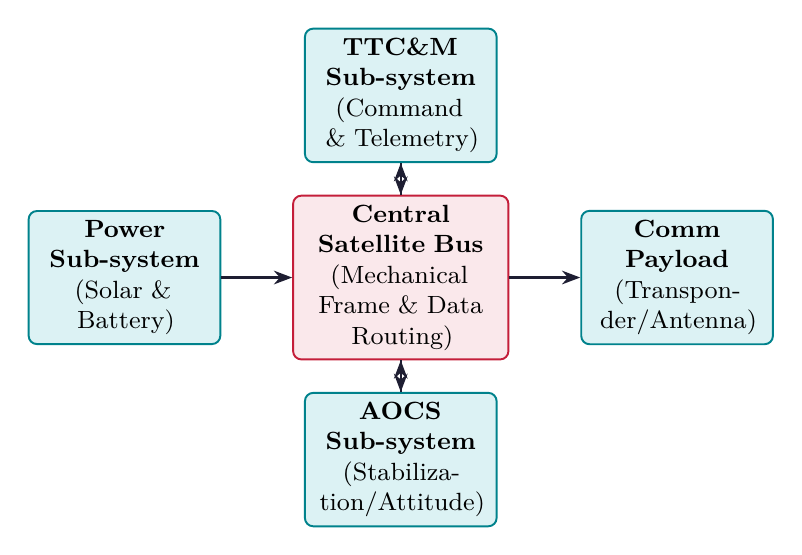
\begin{tikzpicture}[node distance=0.4cm and 0.9cm, every node/.style={font=\scriptsize}]
  % Central integration node
  \node[redblock, text width=2.5cm, minimum height=1.2cm] (bus) {\textbf{Central Satellite Bus}\\(Mechanical Frame \& Data Routing)};
  
  % Surrounding subsystems
  \node[block, above=of bus, text width=2.2cm] (ttcm) {\textbf{TTC\&M Sub-system}\\(Command \& Telemetry)};
  \node[block, below=of bus, text width=2.2cm] (aocs) {\textbf{AOCS Sub-system}\\(Stabilization/Attitude)};
  \node[block, left=of bus, text width=2.2cm] (power) {\textbf{Power Sub-system}\\(Solar \& Battery)};
  \node[block, right=of bus, text width=2.2cm] (payload) {\textbf{Comm Payload}\\(Transponder/Antenna)};
  
  % Interconnections
  \draw[arrow] (ttcm) -- (bus);
  \draw[arrow] (bus) -- (ttcm);
  \draw[arrow] (aocs) -- (bus);
  \draw[arrow] (bus) -- (aocs);
  \draw[arrow] (power) -- (bus);
  \draw[arrow] (bus) -- (payload);
\end{tikzpicture}
\end{tcolorbox}

% ===============================================================================
\section{Telemetry, Tracking, Command, and Monitoring (TTC\&M)}
% ===============================================================================

The TTC\&M sub-system establishes a constant bi-directional radio control link between the satellite and the ground control station (Earth Station).

\begin{itemize}[leftmargin=*, itemsep=3.5pt]
  \item \textbf{Telemetry (Transmission from Space to Earth):} Gathers diagnostic sensor data onboard the satellite (such as battery voltage, solar cell current, internal temperature, and gas pressure) and transmits this status information to Earth.
  \item \textbf{Tracking (Determination of Position):} Measures slant range, angular coordinates, and Doppler shift of the satellite's beacon to compute its precise orbital position, ensuring it has not drifted.
  \item \textbf{Command (Reception from Earth to Space):} Receives control instructions from the ground station to execute tasks like firing thrusters for orbital correction, switching transponder channels, or deploying solar arrays.
  \item \textbf{Monitoring:} Continuous checking of payload performance and checking for anomalies.
\end{itemize}

% ===============================================================================
\section{Attitude and Orbit Control System (AOCS)}
% ===============================================================================

The AOCS is responsible for keeping the satellite in its correct orbital slot (station-keeping) and ensuring its antennas and solar panels are pointing in the correct directions (attitude control).

\begin{itemize}[leftmargin=*, itemsep=4pt]
  \item \textbf{Attitude Control:} Stabilizes the satellite relative to its three axes:
    \begin{itemize}[leftmargin=*, itemsep=2pt, topsep=2pt]
      \item \textbf{Roll:} Rotation around the longitudinal axis (tangent to orbit velocity).
      \item \textbf{Pitch:} Rotation around the lateral axis (perpendicular to orbit plane).
      \item \textbf{Yaw:} Rotation around the vertical axis (pointing toward Earth's center).
    \end{itemize}
  \item \textbf{Orbit Control (Station Keeping):} Fires thrusters to correct long-term orbital drift caused by gravitational pulls from the Sun/Moon, Earth's equatorial asymmetry (ellipticity), and solar radiation pressure.
\end{itemize}

\subsection{Stabilization Techniques}
There are two main methods to keep a satellite from tumbling:
\begin{enumerate}[label=\textbf{\arabic*.}, leftmargin=*, itemsep=2pt]
  \item \textbf{Spin Stabilization:} The satellite body is spun rapidly at 30 to 100 rpm, using gyroscopic momentum to maintain axis alignment. The antennas must be mounted on a "despun" platform rotating in the opposite direction to remain fixed on Earth.
  \item \textbf{Three-Axis (Body) Stabilization:} The satellite body remains fixed relative to Earth. Momentum wheels or reaction wheels inside the satellite spin at varying speeds to absorb and counteract external disturbance torques.
\end{enumerate}

% ===============================================================================
\section{Communication Sub-system: Transponders}
% ===============================================================================

The transponder is the heart of the communication payload. A satellite typical houses 12 to 96 transponders, each acting as a separate channel.

\subsection{Bent-Pipe (Frequency Translation) Transponder}
Also known as a \textbf{repeater transponder}. It simply amplifies the incoming signal, down-converts its frequency, and transmits it. It does not look at or alter the digital content.

\begin{tcolorbox}[tikzbox, title={Bent-Pipe Transponder Block Diagram}]
\centering
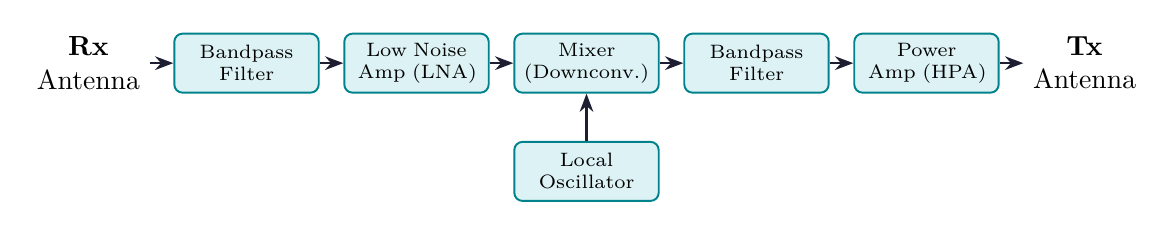
\begin{tikzpicture}[node distance=0.2cm and 0.4cm,
  sblock/.style={rectangle, draw=myteal, fill=hdrteal, text width=1.6cm,
    align=center, minimum height=0.75cm, font=\scriptsize,
    rounded corners=3pt, line width=0.7pt}]
  
  % Nodes
  \node (ant_rx) [align=center] {\textbf{Rx}\\Antenna};
  \node[sblock, right=0.3cm of ant_rx] (bpf1) {Bandpass\\Filter};
  \node[sblock, right=0.3cm of bpf1] (lna) {Low Noise\\Amp (LNA)};
  \node[sblock, right=0.3cm of lna] (mixer) {Mixer\\(Downconv.)};
  \node[sblock, below=0.6cm of mixer] (lo) {Local\\Oscillator};
  \node[sblock, right=0.3cm of mixer] (bpf2) {Bandpass\\Filter};
  \node[sblock, right=0.3cm of bpf2] (hpa) {Power\\Amp (HPA)};
  \node (ant_tx) [right=0.3cm of hpa, align=center] {\textbf{Tx}\\Antenna};
  
  % Arrows
  \draw[arrow] (ant_rx) -- (bpf1);
  \draw[arrow] (bpf1) -- (lna);
  \draw[arrow] (lna) -- (mixer);
  \draw[arrow] (lo) -- (mixer);
  \draw[arrow] (mixer) -- (bpf2);
  \draw[arrow] (bpf2) -- (hpa);
  \draw[arrow] (hpa) -- (ant_tx);
\end{tikzpicture}
\end{tcolorbox}

\begin{itemize}[leftmargin=*, itemsep=3.5pt]
  \item \textbf{Low Noise Amplifier (LNA):} Amplifies the extremely weak uplink signal (in the range of picowatts) while adding minimal thermal noise.
  \item \textbf{Mixer \& Local Oscillator:} Translates the signal frequency. The shift is $\Delta f = f_{LO} = f_u - f_d$ (e.g., $6 \text{ GHz} - 4 \text{ GHz} = 2 \text{ GHz}$).
  \item \textbf{High Power Amplifier (HPA):} Amplifies the downlink signal to several watts using Traveling-Wave Tube Amplifiers (TWTAs) or Solid-State Power Amplifiers (SSPAs) for transmission.
\end{itemize}

\subsection{Regenerative (Demodulation/Remodulation) Transponder}
A regenerative transponder demodulates the incoming analog signal down to the digital baseband bitstream, cleans up the digital noise (performing error correction), and then remodulates the digital data onto a new downlink carrier.
It acts as a \textbf{"computer in space"}, isolating the uplink noise from the downlink path.

% ===============================================================================
\section{Power Sub-system}
% ===============================================================================

The power subsystem must generate, store, regulate, and distribute electrical power.
\begin{itemize}[leftmargin=*, itemsep=3.5pt]
  \item \textbf{Primary Source (Solar Arrays):} Gallium Arsenide (GaAs) or Silicon solar panels convert solar energy into electrical power. In GEO, arrays must continuously track the Sun.
  \item \textbf{Secondary Source (Batteries):} Rechargeable batteries (Nickel-Hydrogen $\text{Ni-H}_2$ or Lithium-Ion) store electrical energy to power the spacecraft during \textbf{solar eclipses} when Earth blocks sunlight.
  \item \textbf{Power Conditioning Unit (PCU):} Regulates the bus voltage (typically 28V, 50V, or 100V DC) and controls battery charging/discharge rates.
\end{itemize}

% ===============================================================================
% MANDATORY QUICK REVISION PAGE
% ===============================================================================
\newpage
\begin{center}
  {\large\bfseries\color{myred} Quick Revision --- Module III}\\[3pt]
  {\small\color{mydark} Satellite Sub-systems $|$ PE-EC701B}
\end{center}
\noindent{\color{myred}\rule{\linewidth}{1.2pt}}
\vspace{4pt}

\begin{tcolorbox}[formulabox, title={\textbf{Key Formulas at a Glance}}]
\renewcommand{\arraystretch}{1.3}
\begin{tabularx}{\linewidth}{B{5.0cm} X}LO Frequency Shift & $f_{LO} = f_{uplink} - f_{downlink}$ \\[4pt]
Solar Panel Efficiency & $P = \eta \cdot S \cdot A \cdot \cos(\theta)$ \quad ($S \approx 1367 \text{ W/m}^2$, $\eta$ = efficiency) \\[4pt]
Battery Capacity & $C_{req} = \frac{P_{load} \times t_{eclipse}}{DoD \times V_{bus}}$ \quad ($DoD$ = Depth of Discharge) \\[4pt]
Local Oscillator Shift (C-Band) & $f_{LO} = 5.925\text{ GHz} - 3.7\text{ GHz} = 2.225\text{ GHz}$
\end{tabularx}
\tcbset{colbacktitle=myteal, coltitle=white}
\end{tcolorbox}

\begin{tcolorbox}[defbox, title={\textbf{One-Line Definitions}}]
\begin{itemize}[leftmargin=*, itemsep=2.5pt, topsep=0pt]
  \item \textbf{TTC\&M:} Ground station radio link monitoring health, status, and position of the satellite.
  \item \textbf{AOCS:} The subsystem stabilizing satellite orientation and correcting orbital drift.
  \item \textbf{Bent-Pipe Transponder:} A simple frequency translation and amplification transponder.
  \item \textbf{Regenerative Transponder:} A transponder that demodulates, processes, and remodulates data.
  \item \textbf{Despun Platform:} A platform rotating oppositely to a spin-stabilized satellite body to keep antennas fixed.
  \item \textbf{Reaction Wheels:} Internal motor-driven wheels adjusting satellite attitude via conservation of angular momentum.
  \item \textbf{Station Keeping:} Maneuvers using thrusters to keep a satellite within its assigned orbital box.
\end{itemize}
\end{tcolorbox}

\begin{tcolorbox}[exambox, title={\textbf{Frequently Asked / Viva Questions}}]
\begin{enumerate}[topsep=0pt, label=\textbf{Q\arabic*.}, itemsep=5pt]
  \item \Q{Differentiate between satellite payload and satellite bus.}
    The payload represents the hardware performing the actual service (transponders and antennas). The bus represents the supporting infrastructure (structure, power, thermal, AOCS, TTC\&M).
  \item \Q{What are the functions of Telemetry and Command in TTC\&M?}
    Telemetry transmits internal sensor readings (health data) from the satellite to Earth. Command receives control signals from Earth to execute adjustments inside the satellite.
  \item \Q{Explain the three attitude axes of a satellite: Roll, Pitch, and Yaw.}
    Roll: rotation about the velocity vector. Pitch: rotation perpendicular to the orbit plane. Yaw: rotation pointing directly toward the center of the Earth.
  \item \Q{Compare Spin Stabilization and Three-Axis Stabilization.}
    Spin stabilization uses gyroscopic spin of the entire body to maintain axis alignment. Three-axis stabilization keeps the outer body stationary while internal reaction wheels spin dynamically to absorb disturbance torques.
  \item \Q{Draw the basic block diagram of a bent-pipe transponder.}
    Rx Antenna $\to$ BPF $\to$ LNA $\to$ Mixer (with LO) $\to$ BPF $\to$ HPA $\to$ Tx Antenna.
  \item \Q{Why is an LNA placed as the first block in the transponder receiver chain?}
    Because the received uplink signal is extremely weak. Amplifying it first with a Low Noise Amplifier establishes a high signal-to-noise ratio, preventing subsequent stages from corrupting the signal.
  \item \Q{What is the advantage of a regenerative transponder over a bent-pipe transponder?}
    It demodulates and decodes the signal, stripping away uplink noise and distortion. It then regenerates and remodulates the clean digital bits, preventing noise accumulation.
  \item \Q{Why do satellites require battery systems if they have solar panels?}
    Because satellites periodically pass through the Earth's shadow (solar eclipses) where solar panels cannot generate power. Batteries provide secondary power during these shadow periods.
  \item \Q{What is the function of the thrusters in the propulsion system?}
    To perform station-keeping (correcting orbital drift caused by Sun/Moon gravity) and attitude adjustments when reaction wheels saturate.
  \item \Q{What is Depth of Discharge (DoD) in satellite batteries?}
    It is the percentage of battery capacity used during an eclipse. Satellites restrict DoD to 50--80\% to maximize the operational lifespan of the batteries.
  \item \Q{Why is thermal control critical in spacecraft design?}
    In vacuum, heat is only transferred by radiation. The side facing the Sun heats to $>100^\circ\text{C}$ while the shadow side drops to $<-100^\circ\text{C}$. The thermal system redistributes heat to keep electronics in operational ranges.
  \item \Q{What is a local oscillator frequency offset, and how is it chosen?}
    It is chosen to match the frequency separation between uplink and downlink bands (e.g., 2.225 GHz offset for C-band) to prevent electromagnetic feedback.
\end{enumerate}
\end{tcolorbox}

\begin{tcolorbox}[tikzbox, title={Comparison of Transponder Architectures}]
\renewcommand{\arraystretch}{1.4}
\par\noindent
{\renewcommand{\arraystretch}{1.55}%
\begin{tabularx}{\linewidth}{|B{3.2cm}|Y|Y|}\hline
\textbf{Feature} & \textbf{\color{myteal}Bent-Pipe Transponder} & \textbf{\color{mypurple}Regenerative Transponder} \\[4pt]
\hline
\textbf{Basic Operation} & RF-to-RF translation & Demodulation $\to$ Baseband Processing $\to$ Remodulation \\[4pt]
\hline
\textbf{Noise Propagation} & Uplink noise is amplified and sent down. & Uplink noise is removed at baseband. \\[4pt]
\hline
\textbf{Complexity \& Weight} & Low complexity, lightweight, highly reliable. & High complexity, heavy, requires onboard processors. \\[4pt]
\hline
\textbf{Flexibility} & Protocol transparent (handles any modulation format). & Protocol-specific (locked to a particular modulation/coding standard). \\[4pt]
\hline
\textbf{Primary Use Case} & Standard satellite TV distribution, VSAT links. & Modern satellite broadband, military secure links. \\[4pt]
\hline
\end{tabularx}
}
\end{tcolorbox}

\end{document}
